\documentclass{beamer}
\usetheme{ConnectivityLab}
\usepackage{times}
\usepackage{graphicx}
\usepackage{verbatim}
\usepackage{outlines}
\usepackage{fancyhdr}
\usepackage{subfigure}
\usepackage{cancel}
\usepackage{bibentry}
\usepackage{varwidth}
\usepackage{etoolbox}
\usepackage{epstopdf}

%%%%%%%%%%%%%%%%%%%%%%%%%%%%%%%%%%%%%%%%%%%%%%%%%%%%%%
%%%%%%%%%%%%%%%%%%%%%%%%%%%%%%%%%%%%%%%%%%%%%%%%%%%%%%

\title {
    Security, Privacy, and Fairness in Fog-Based Vehicular Crowdsensing\cite{JNI2017}
}
\author {
    Yin-Hong Hsu
}
\date {
    03 02, 2018
}

%%%%%%%%%%%%%%%%%%%%%%%%%%%%%%%%%%%%%%%%%%%%%%%%%%%%%%
%%%%%%%%%%%%%%%%%%%%%%%%%%%%%%%%%%%%%%%%%%%%%%%%%%%%%%

\begin{document}
\begin{frame}
    \titlepage
\end{frame}

%%%%%%%%%%%%%%%%%%%%%%%%%%%%%%%%%%%%%%%%%%%%%%%%%%%%%%
%%%%%%%%%%%%%%%%%%%%%%%%%%%%%%%%%%%%%%%%%%%%%%%%%%%%%%

\begin{frame}{Outline}
    \tableofcontentsgather
    \tableofcontents
\end{frame}

%%%%%%%%%%%%%%%%%%%%%%%%%%%%%%%%%%%%%%%%%%%%%%%%%%%%%%
%%%%%%%%%%%%%%%%%%%%%%%%%%%%%%%%%%%%%%%%%%%%%%%%%%%%%%
\section{Intorduction}
\begin{frame}{Intorduction}
    \begin{itemize}
        \item {A study of security, privacy, fairness requirements in fog-based vehicle crowdsensing}
        \item {And discuss the possible solutions}
        \item {Fog-based vehicle crowdsensing (FVCS) can provide local services (e.g., real-time nevigation, parking space reservation)}
    \end{itemize}
\end{frame}
\section{Architecture}
\begin{frame}{Architecture}
    \begin{figure}[t]
        \centering
        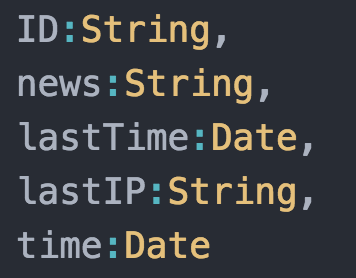
\includegraphics[width=1.0\textwidth]{figures/1.png}
        
    \end{figure}
\end{frame}
\section{Challenges}
\begin{frame}{Challenges - Security}
    \begin{itemize}
        \item {Malicious hacker might extract personal info from the intersaction of multiple crowdsensing report}
        \item {In authentication issue, the blacklist should be built to resist impersonation attacks and Sybil attacks}
    \end{itemize}
\end{frame}
\begin{frame}{Challenges - Privacy}
    \begin{itemize}
        \item {The sensing data are related to people-centric information, also included where driver and passenger are goin or what place they frequently visit}
        \item {The more promising method to protect vehicles' privacy is to use anonymity technology (e.g., group signature, k-anonymity)}
    \end{itemize}
\end{frame}
\begin{frame}{Challenges - Fairness}
    \begin{itemize}
        \item {How to guarantee the fairness of vehicles is dramatically critaical}
        \item {The data sensed from same position inevitably contain some duplicates, which may waste massive bandwidth and storage}
        \item {It is necessary to design a verifiable reward distribution mechanism for vehicles to ensure their fairness}
    \end{itemize}
\end{frame}
\section{Solution}
\begin{frame}{Solution - Security}
    \begin{itemize}
        \item {A Trusted Authority (TA) should be involved to achieve key management}
    \end{itemize}
    \begin{figure}[t]
        \centering
        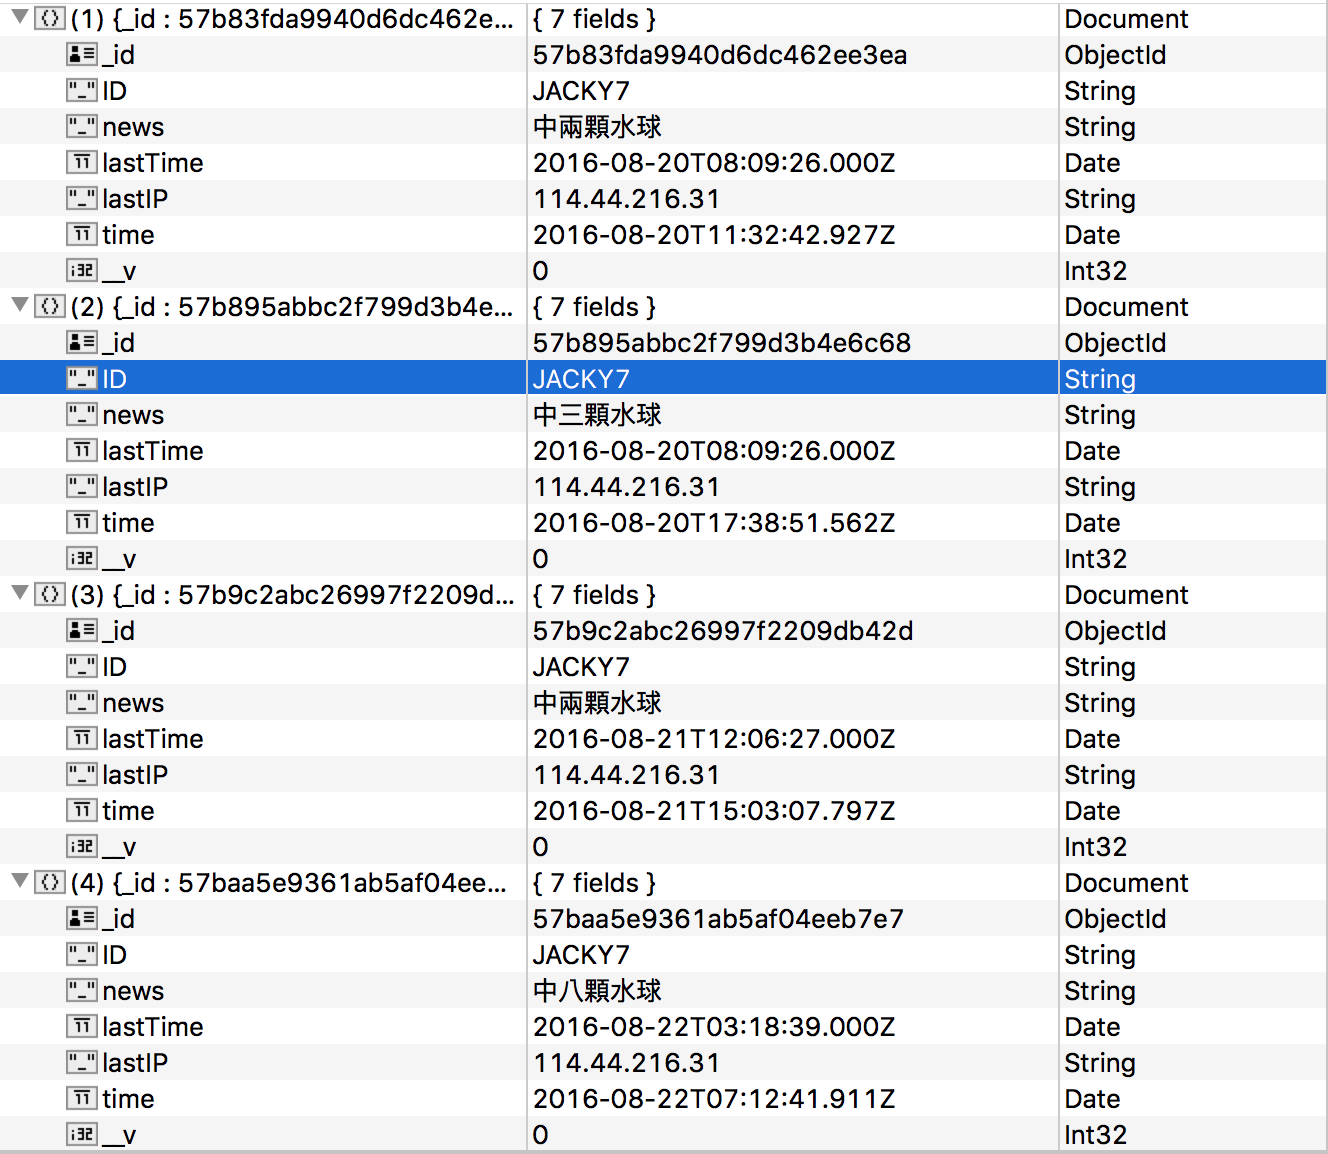
\includegraphics[width=0.6\textwidth]{figures/2.png}
    \end{figure}
\end{frame}
\begin{frame}{Solution - Privacy}
    \begin{itemize}
        \item {Use signature generated by TA to accomplish privacy requirement}
    \end{itemize}
    \begin{figure}[t]
        \centering
        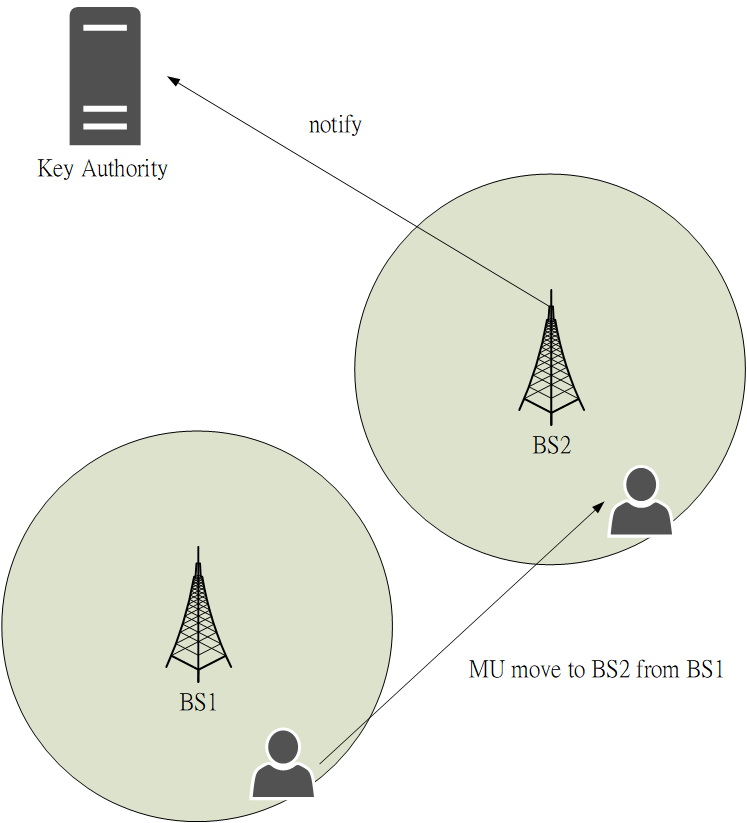
\includegraphics[width=0.9\textwidth]{figures/3.png}
    \end{figure}
\end{frame}
\begin{frame}{Solution - Fairness}
    \begin{itemize}
        \item {The straightforward method is to discard the duplicate data; however, to disclose the sensing report will leak personal information}
    \end{itemize}
    \begin{figure}[t]
        \centering
        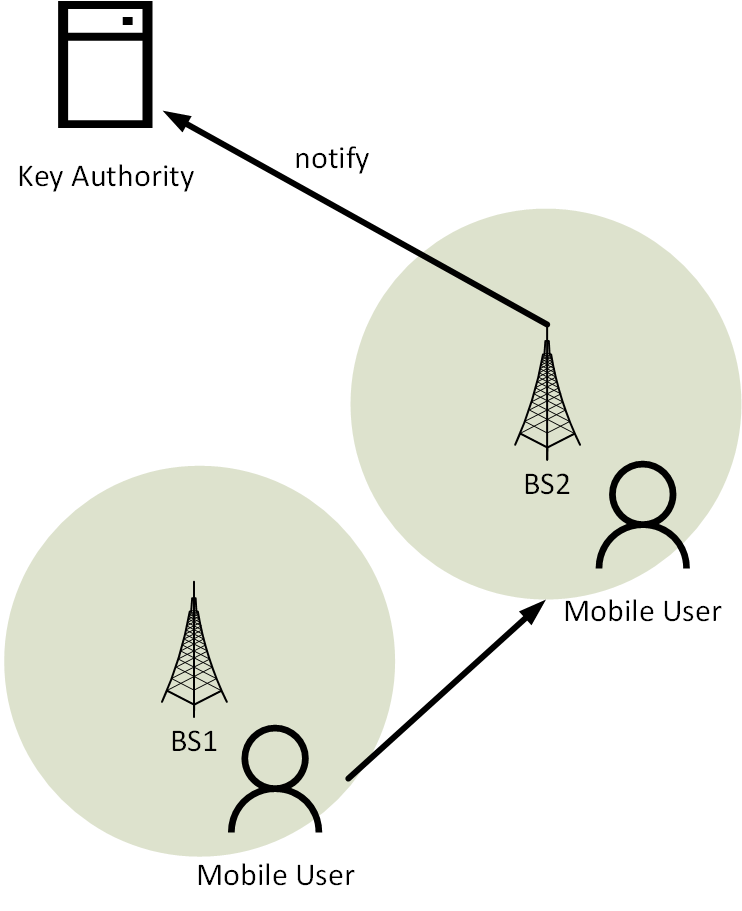
\includegraphics[width=0.8\textwidth]{figures/4.png}
    \end{figure}
\end{frame}
%%%%%%%%%%%%%%%%%%%%%%%%%%%%%%%%%%%%%%%%%%%%%%%%%%%%%%
%%%%%%%%%%%%%%%%%%%%%%%%%%%%%%%%%%%%%%%%%%%%%%%%%%%%%%

\section{References}
\calcreferencespagetotal % Calc your References Page total number
\begin{frame}[allowframebreaks]{References}
    \fontsize{9pt}{13}\selectfont
    \bibliographystyle{IEEEtran}
    \bibliography{IEEEabrv,Citation}
\end{frame}

%%%%%%%%%%%%%%%%%%%%%%%%%%%%%%%%%%%%%%%%%%%%%%%%%%%%%%
%%%%%%%%%%%%%%%%%%%%%%%%%%%%%%%%%%%%%%%%%%%%%%%%%%%%%%
\section{}

\begin{frame}
    \centering
    \Large{Thanks for Your Attentions}
\end{frame}

\end{document}
